\begin{frame}{Attack Outline}

\begin{itemize}
    \item \textbf{Guess} some bits in a few successive states.
    \begin{itemize}
          \item<2-> Least-significant bits
          \item<2-> Rotations
    \end{itemize}
      
    \medskip
      
    \item[$\Rightarrow$] Turn it into a \textbf{(regular) truncated congruential generator}.
      
    \medskip

    \item \textbf{Reconstruct} hidden information using lattice techniques.
    \begin{itemize}
          \item<3-> Easy case: full state
          \item<3-> Hard case: partial information (next rotations)
      \end{itemize}
    
    \medskip
    
    \item \textbf{Discard} bad guesses.
\end{itemize}
\end{frame}



\begin{frame}{Easy Case: Known increment}

If the \alert{increment} (\alert{c}) is \textbf{known}...

\bigskip

\begin{exampleblock}{... Get rid of it!}
\begin{itemize}
    \item $S'_0 \gets S_0$
    \item $S'_1 \gets S_1 - c$
    \item $S'_2 \gets S_2 - (a+1)c$
    \item $S'_3 \gets S_3 - (a^2 + a + 1)c$
    \item $\vdots$
\end{itemize}
\end{exampleblock}

\bigskip

Yields $S' :$ sequence of states with $c=0$ (geometric sequence).

\end{frame}



\begin{frame}[label=atk_details]{Attack Details}

\begin{figure}
\begin{center}
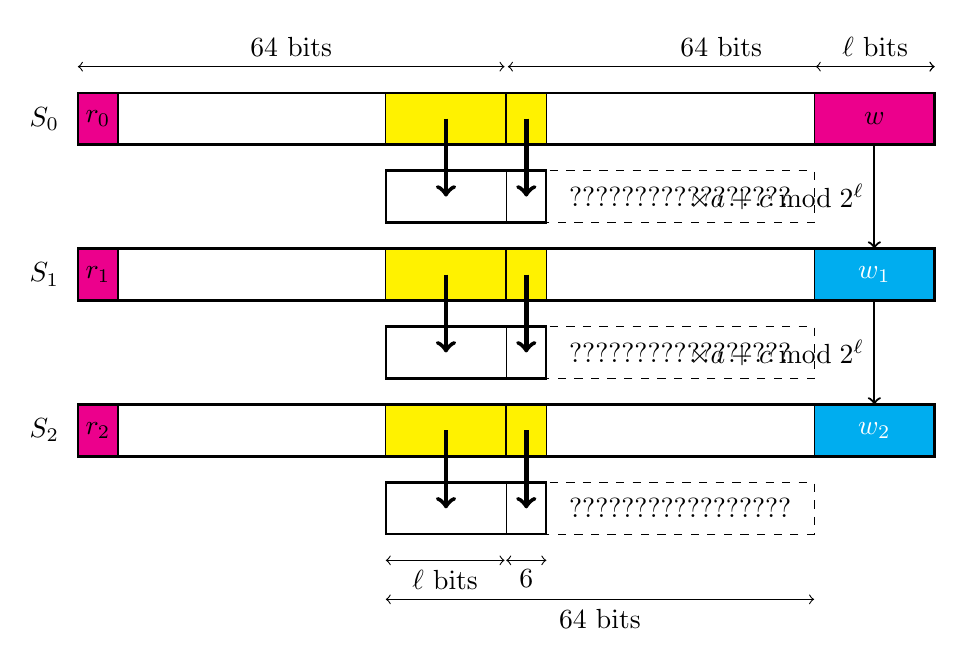
\begin{tikzpicture}[xscale=0.85, yscale=0.66]
  \path[red, use as bounding box] (-0.75, -9.5) rectangle (12.8, 2.25);
  
  % S_0
  \begin{scope}
    % remplissage
    \fill<4-5>[fill=yellow] (4.6, 0) rectangle +(2.4, 1);
    \fill<2-5>[fill=magenta] (0, 0) rectangle node {$r_0$} +(0.6, 1);
    \fill<2-5>[fill=magenta] (11, 0) rectangle node {$w$} +(1.8, 1);
    
    % bordures
    \draw<1-5>[thick]  (0, 0) rectangle (12.8, 1);
    \draw<2-5>  (0.6, 0) rectangle +(0, 1);
    \draw<1-5>[thick]  (6.4, 0) rectangle +(0, 1);
    \draw<4-5>  (7.0, 0) rectangle +(0, 1);
    \draw<4-5> (4.6, 0) rectangle +(0, 1);
    \draw<2-5>  (11, 0) rectangle +(0, 1);
    
    % déco autour
    \node<1-5> at (-0.5, 0.5) {$S_0$};
    \draw<1-5>[<->] (0, 1.5) -- node[above] {64 bits} +(6.375, 0);
    \draw<1>[<->] (6.425, 1.5) -- node[above] {64 bits} +(6.375, 0);
    \draw<2-5>[<->] (12.8, 1.5) -- node[above] {$\ell$ bits} +(-1.775, 0);
  \end{scope}

  % T_0
  \begin{scope}[xshift=4.6cm, yshift=-1.5cm]    
    \draw<5->[dashed]  (0, 0) rectangle +(6.4, 1);
    \draw<5->[thick]   (0, 0) rectangle +(2.4, 1);
    \draw<5>[]   (1.8, 0) rectangle +(0, 1);
    \path<5->  (2.4, 0) rectangle node {$?????????????????$} (6.4, 1);
  \end{scope}

  % flèches S_i --> T_i
  \draw<5> [ultra thick,->] (5.5, 0.5) -- +(0, -1.5);
  \draw<5> [ultra thick,->] (6.7, 0.5) -- +(0, -1.5);

  
  %%%%%%%%%

  
  % S_1
  \begin{scope}[yshift=-3cm]
    % remplissage
    \fill<4-5>[fill=yellow] (4.6, 0) rectangle +(2.4, 1);
    \fill<2-5>[fill=magenta] (0, 0) rectangle node {$r_1$} +(0.6, 1);
    \fill<3-5>[fill=cyan] (11, 0) rectangle node[text=white] {$w_1$} +(1.8, 1);
    
    % bordures
    \draw<1-5>[thick]  (0, 0) rectangle (12.8, 1);
    \draw<2-5>  (0.6, 0) rectangle +(0, 1);
    \draw<1-5>[thick]  (6.4, 0) rectangle +(0, 1);
    \draw<4-5>  (7.0, 0) rectangle +(0, 1);
    \draw<4-5>  (4.6, 0) rectangle +(0, 1);
    \draw<3-5>  (11, 0) rectangle +(0, 1);
    
    % déco autour
    \node<1-5> at (-0.5, 0.5) {$S_1$};

    % flèches S_i --> T_i
    \draw<5>[ultra thick,->] (5.5, 0.5) -- +(0, -1.5);
    \draw<5>[ultra thick,->] (6.7, 0.5) -- +(0, -1.5);
  \end{scope}

  % T_1
  \begin{scope}[xshift=4.6cm, yshift=-4.5cm]    
    \draw<5->[dashed]  (0, 0) rectangle +(6.4, 1);
    \draw<5->[thick]  (0, 0) rectangle +(2.4, 1);
    \draw<5>[]  (1.8, 0) rectangle +(0, 1);
    \path<5-> (2.4, 0) rectangle node {$?????????????????$} (6.4, 1);
  \end{scope}

  %%%%%%%%%%%%%

  
  % S_2
  \begin{scope}[yshift=-6cm]
    % remplissage
    \fill<4-5>[fill=yellow] (4.6, 0) rectangle +(2.4, 1);
    \fill<2-5>[fill=magenta] (0, 0) rectangle node {$r_2$} +(0.6, 1);
    \fill<3-5>[fill=cyan] (11, 0) rectangle node[text=white] {$w_2$} +(1.8, 1);
    
    % bordures
    \draw<1-5>[thick]  (0, 0) rectangle (12.8, 1);
    \draw<2-5>  (0.6, 0) rectangle +(0, 1);
    \draw<1-5>[thick]  (6.4, 0) rectangle +(0, 1);
    \draw<4-5>  (7.0, 0) rectangle +(0, 1);
    \draw<4-5>  (4.6, 0) rectangle +(0, 1);
    \draw<3-5>  (11, 0) rectangle +(0, 1);
    
    % déco autour
    \node<1-5> at (-0.5, 0.5) {$S_2$};
    
    % flèches S_i --> T_i
    \draw<5>[ultra thick,->] (5.5, 0.5) -- +(0, -1.5);
    \draw<5>[ultra thick,->] (6.7, 0.5) -- +(0, -1.5);
  \end{scope}

  % T_2
  \begin{scope}[xshift=4.6cm, yshift=-7.5cm]    
    \draw<5->[dashed]  (0, 0) rectangle +(6.4, 1);
    \draw<5->[thick]  (0, 0) rectangle +(2.4, 1);
    \draw<5>[]  (1.8, 0) rectangle +(0, 1);
    \path<5-> (2.4, 0) rectangle node {$?????????????????$} (6.4, 1);

    % déco
    \draw<5->[<->] (0, -0.5) -- node[below] {$\ell$ bits} +(1.775, 0);
    \draw<5->[<->] (1.8, -0.5) -- node[below] {6} +(0.6, 0);
    \draw<6->[<->] (0, -1.25) -- node[below] {64 bits} +(6.4, 0);
  \end{scope}

  % flèches w
  \draw<3>[thick,->] (11.9, 0) -- node[left] {$\times a + c \bmod \alert{2^\ell}$} +(0, -2);
  \draw<3>[thick,->] (11.9, -3) -- node[left] {$\times a + c \bmod \alert{2^\ell}$} +(0, -2);
  

\end{tikzpicture}
\end{center}
\end{figure}

\end{frame}

%%%%%%%%%%%%%%

\begin{frame}[label=atk_details]{Remove the ``Constant Component''}

\begin{center}
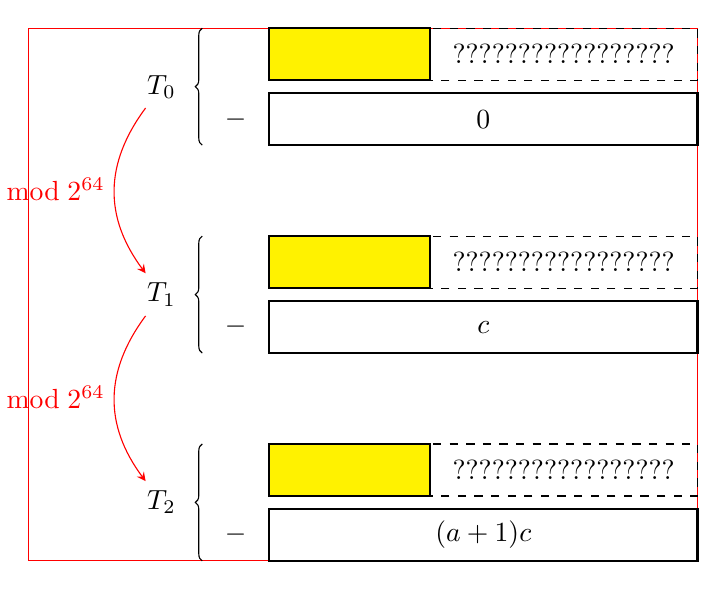
\begin{tikzpicture}[xscale=0.85, yscale=0.66, decoration={brace,mirror},>=stealth]
  \draw[red, use as bounding box] (1, -10.75) rectangle (11, -0.5);
  
  % T_0
  \begin{scope}[xshift=4.6cm, yshift=-1.5cm]    
    \draw[dashed]  (0, 0) rectangle +(6.4, 1);
    \draw[thick,fill=yellow]   (0, 0) rectangle +(2.4, 1);
    %\draw[]   (1.8, 0) rectangle +(0, 1);
    \path  (2.4, 0) rectangle node {$?????????????????$} (6.4, 1);

    % déco
    \draw[decorate]  (-1, 1) -- +(0, -2.25);
    \node[anchor=east] at (-1.25, -0.125)  (T0) {$T_0$};
  \end{scope}

  % composante en c 0
  \begin{scope}[xshift=4.6cm, yshift=-2.75cm]    
  \draw[thick]  (0, 0) rectangle node {$0$} +(6.4, 1);
  \node  at (-0.5, 0.5) {$-$};
  \end{scope}

  % T_1
  \begin{scope}[xshift=4.6cm, yshift=-5.5cm]    
    \draw[dashed]  (0, 0) rectangle +(6.4, 1);
    \draw[thick,fill=yellow]  (0, 0) rectangle +(2.4, 1);
    %\draw[]  (1.8, 0) rectangle +(0, 1);
    \path (2.4, 0) rectangle node {$?????????????????$} (6.4, 1);

    % déco
    \draw[decorate]  (-1, 1) -- +(0, -2.25);
    \node[anchor=east] at (-1.25, -0.125)  (T1) {$T_1$};
  \end{scope}

  % composante en c 1
  \begin{scope}[xshift=4.6cm, yshift=-6.75cm]    
  \draw[thick]  (0, 0) rectangle node {$c$} +(6.4, 1);
  \node  at (-0.5, 0.5) {$-$};
  \end{scope}


  % T_2
  \begin{scope}[xshift=4.6cm, yshift=-9.5cm]    
    \draw[dashed]  (0, 0) rectangle +(6.4, 1);
    \draw[thick,fill=yellow]  (0, 0) rectangle +(2.4, 1);
    %\draw[]  (1.8, 0) rectangle +(0, 1);
    \path (2.4, 0) rectangle node {$?????????????????$} (6.4, 1);

    % déco
    \draw[decorate]  (-1, 1) -- +(0, -2.25);
    \node[anchor=east] at (-1.25, -0.125) (T2) {$T_2$};
  \end{scope}

    % composante en c 2
  \begin{scope}[xshift=4.6cm, yshift=-10.75cm]    
  \draw[thick]  (0, 0) rectangle node {$(a+1)c$} +(6.4, 1);
  \node  at (-0.5, 0.5) {$-$};
  \end{scope}

  
  % arrows
  \draw[red,->] (T0) edge[bend right] node[left] {$\times a \bmod 2^{64}$} (T1);
  \draw[red,->] (T1) edge[bend right] node[left] {$\times a \bmod 2^{64}$} (T2);
  
\end{tikzpicture}
\end{center}

\end{frame}


%%% Local Variables:
%%% mode: latex
%%% TeX-master: "../main.tex"
%%% End:
